\section{安全用电}\label{sec:11-4}

利用电能,可以提高生产效率,改善生活条件,但是必须注意安全,否则可能引起火灾或者造成触电事故。

触电时有电流通过人体,但是有电流通过人体并不都会发生触电事故。
两手分别触摸一节干电池的正负极,有电流通过人体,人并没有不舒服的感觉,原因是电流非常弱。
1 毫安左右的电流通过人体就会引起麻的感觉,但不超过 10 毫安左右时,触电人自己可以摆脱电源,不致造成事故。
超过 30 毫安时,会使人感到剧痛甚至神经麻痹、呼吸困难,有生命危险。
达到 100 毫安,只要很短的时间就会使呼吸窒息,心跳停止。
电流越强,从触电到死亡的时间越短。

通过人体的电流强度决定于外加电压和人体的电阻。
人体的电阻不是每个人都一样大,同一个人也不是固定不变的,皮肤干燥的时候大些,潮湿的时候小些。
所以绝不可因为某人接触过某一电压没有伤亡,就认为这样的电压对任何人都安全,
也不可因为自己接触过某一电压没有出事,就以为这样的电压对自己总是安全的。

经验证明,\textbf{只有不高于 36 伏特的电压才是安全的}。

照明电路的电压是 220 伏特,动力电路的电压是 380 伏特,这些电路在电工技术中虽然都叫做低压线路,
但都高出安全电压很多。高压线路的电压高达几十千伏甚至几百千伏,更是远远超出安全电压。

照明电路引起的触电事故,都是由于人体直接或间接跟火线连通造成的。什么是火线呢?

照明电路的两根导线中有一根连着地,叫零线(正常情况下零线跟地之间没有电压),
另一根与零线之间有 220 伏特的电压,这根线就叫火线,火线与地之间也有 220 伏特的电压。
辨别零线和火线可以用测电笔(图 \ref{fig:11-8})来测。
测的时候,用手接触笔尾的金属体,笔尖接触电线(或与电线连通的导体),
氖管发光,表明接触的是火线,氖管不发光,表明接触的是零线。

\begin{figure}[htbp]
    \centering
    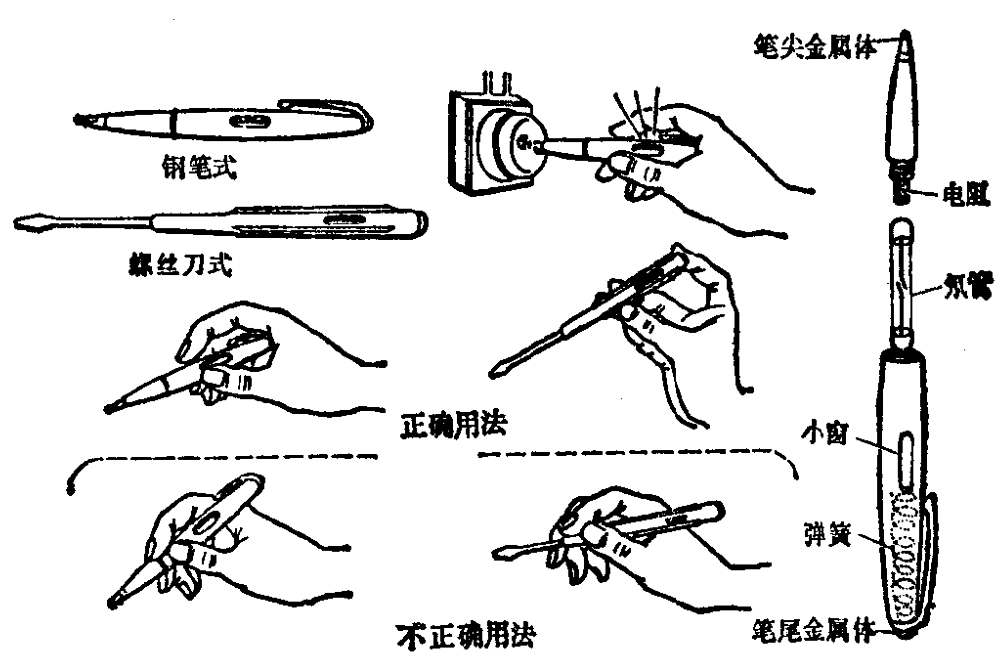
\includegraphics[width=0.9\textwidth]{../pic/czwl2-ch11-8}
    \caption{测电笔的构造和使用方法}\label{fig:11-8}
\end{figure}


站在地上的人触到火线(图 \ref{fig:11-9} 甲),或者站在绝缘体上而同时触到两根电线(图 \ref{fig:11-9} 乙),
就有电流流过人体,造成触电事故。

\begin{figure}[htbp]
    \centering
    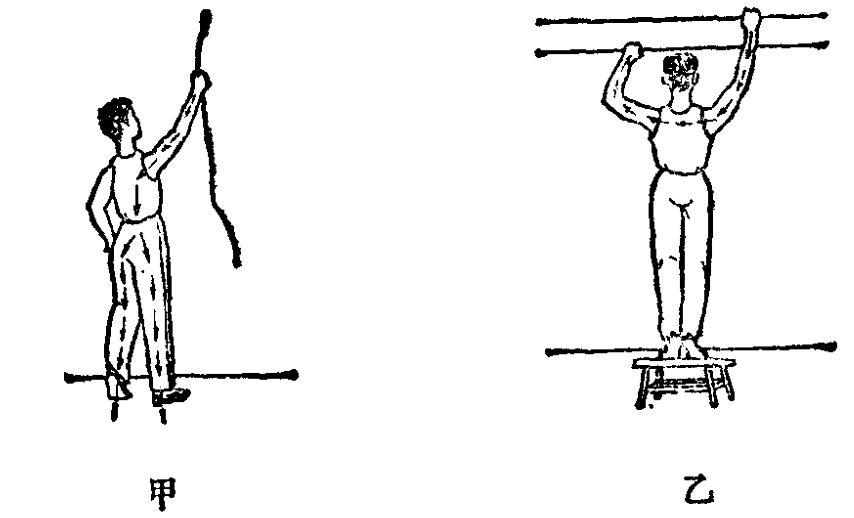
\includegraphics[width=0.7\textwidth]{../pic/czwl2-ch11-9}
    \caption{}\label{fig:11-9}
\end{figure}

高压线路和高压设备引起的触电,有高压电弧触电和跨步电压触电两类。
当人体靠近高压带电体到一定距离时,高压带电体和人体之间就发生放电现象,电流流过人体造成高压电弧触电。
高压输电线落在地面上,当人走近断头时,两脚站在离落地电线远近不同的位置上,两脚之间就存在电压,
电流流过人体,造成跨步电压触电(图 \ref{fig:11-10})。
因此当电线落在地上时,不要靠近,更不能用手去拣,应该派人看守,并赶快找电工处理。

\begin{figure}[htbp]
    \centering
    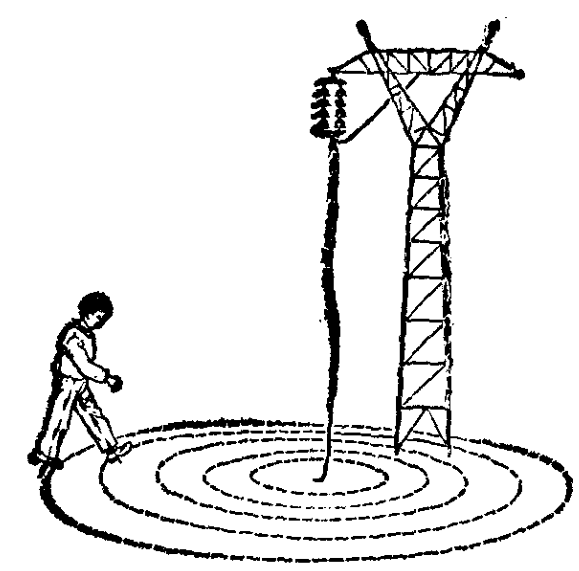
\includegraphics[width=0.6\textwidth]{../pic/czwl2-ch11-10}
    \caption{}\label{fig:11-10}
\end{figure}

了解了触电原因也就懂得了安全用电的原则:\CJKunderwave*{不接触低压带电体,不靠近高压带电体}。
显然这里所说的低压不包括 36 伏特以下的安全电压。

在日常用电中,需要特别警惕的是\CJKunderwave*{本来不应该带电的物体带了电,本来应该绝缘的物体导了电}。
因此该注意:

(1) \CJKunderwave{防止绝缘部分破损}\quad
电线的绝缘皮容易磨损,灯座、插座的绝缘壳容易碰裂,都要注意保护。
台灯、电风扇等常常搬动的设备,它们的电线、插头更要加意保护,并且搬动时要切断电源。

(2) \CJKunderwave{保持绝缘部分干燥}\quad
好的绝缘体潮湿了也会漏电,所以要经常保持电气设备干燥,不使它们的绝缘部分沾水,受潮。
由于水能导电,所以不要用湿手扳开关,不要用湿抹布擦电灯泡,更不能在电线上晾衣服。

(3) \CJKunderwave{避免电线跟其他金属物接触}\quad
架空输电线路的电线是裸线,电话线、广播线、收音机天线、晾衣服铁丝等等,
都应该离架空电线远一些,免得万一暴风雨中电线断开落在这些金属物上,使它们带了电而引起人身触电和设备损坏。
室内的电线虽然有绝缘皮,但是也不要跟金属物连在一起,例如不要挂在铁丝上,免得万一绝缘皮破了铁丝也带了电。

(4) \CJKunderwave*{要定期检查,及时修理}\quad
电气设备用久了,绝缘部分必然老化,难免破损。
为了保证安全,应该由电工定期检查,发现了毛病要及时修理。

还有一点要特别注意的是:当发现有人触电时,应赶快拉断开关或用干燥木棍、竹杆将电线挑开(绝不能空手去拉),
迅速使触电人脱离电源,立即用正确的人工呼吸法进行现场抢救。
发生火灾时,也是要首先拉断开关,切断电源,绝不要带电泼水救火。

掌握了安全用电的知识,严格按照安全用电的要求去做,就可以让电驯服地为我们伟大社会主义祖国的现代化贡献力量。

